\documentclass[7pt]{article}
\usepackage{tree-dvips}
\usepackage[a4paper, total={7.5in, 10.5in}]{geometry}
\usepackage{newunicodechar}
\usepackage{tikz}
\usepackage{tikzpagenodes}
\usepackage{graphicx}
\graphicspath{ {./images/} }
\usepackage{array}
\usepackage{caption}
\captionsetup{labelformat=empty}
\usepackage{float}
\usepackage{boldline}
\newcolumntype{M}[1]{>{\centering\arraybackslash}m{#1}} % center vertical
\newcommand*\circled[1]{\tikz[baseline=(char.base)]{
            \node[shape=circle,draw,inner sep=1.2pt] (char) {#1};}}

\renewcommand{\familydefault}{\sfdefault}
\renewcommand{\arraystretch}{1.65}
\setlength{\arrayrulewidth}{1.5pt}
\pagenumbering{gobble}

\tikzset{
    use page relative coordinates/.style={
        shift={(current page.south west)},
        x={(current page.south east)},
        y={(current page.north west)}
    },
}



\begin{document}
\begin{center}

\end{center}
\begin{tikzpicture}[remember picture,overlay,shift={(current page.north west)}]
\node[anchor=north west,xshift=0.4cm,yshift=-0.4cm]{
\includegraphics[scale=0.3]{images/markerTL.png}};
\end{tikzpicture}
\begin{tikzpicture}[remember picture,overlay,shift={(current page.north east)}]
\node[anchor=north east,xshift=-0.4cm,yshift=-0.4cm]{
\includegraphics[scale=0.3]{images/markerTR.png}};
\end{tikzpicture}

% frame around
%\begin{tikzpicture}[remember picture, overlay,use page relative coordinates]
%\draw[line width=0.8mm] (0.02,0.02) -- (0.98,0.02)  -- (0.98,0.98)  -- (0.02,0.98) -- cycle;
%\end{tikzpicture}

\def\tablebreak{0.5cm}
\def\tablebreakTwo{0.25cm}

\begin{tikzpicture}[remember picture,overlay,shift={(current page.north east)}]
\node[anchor=north east,xshift=-16.6cm,yshift=-2.4cm]{
\includegraphics[scale=0.25]{images/pion.png}};
\end{tikzpicture}

\def\dots{...........................}

% index number table
\begin{table}
  \centering
  \caption{Numer indeksu:\textcolor{white}{.............................} Grupa:}
  \begin{tabular}{M{4.5cm}|M{\tablebreak}|M{\tablebreak}|M{\tablebreak}|M{\tablebreak}|M{\tablebreak}|M{\tablebreak}|M{\tablebreak}|M{\tablebreak} | l{4.5cm}}
    \cline{2-9}
    &  &  &  &  &  &  &  &  & \textbf{INSTRUKCJA} \\ \cline{2-7} \cline{9-9}
    & \circled{0} & \circled{0} & \circled{0} & \circled{0} & \circled{0} & \circled{0} &  & \circled{A} & Poprawnie zaznaczona odpowiedź: \\ \cline{2-7} \cline{9-9}
    & \circled{1} & \circled{1} & \circled{1} & \circled{1} & \circled{1} & \circled{1} &  &  \circled{B} & \\ \cline{2-7} \cline{9-9}
    & \circled{2} & \circled{2} & \circled{2} & \circled{2} & \circled{2} & \circled{2} &  &  \circled{C} & \\ \cline{2-7} \cline{9-9}
    & \circled{3} & \circled{3} & \circled{3} & \circled{3} & \circled{3} & \circled{3} &  & \circled{D} & \\ \cline{2-7} \cline{9-9}
    & \circled{4} & \circled{4} & \circled{4} & \circled{4} & \circled{4} & \circled{4} &  &  & \\ \cline{2-7} \cline{9-9}
    Imię: \dots........ & \circled{5} & \circled{5} & \circled{5} & \circled{5} & \circled{5} & \circled{5} &  &  & Niepoprawnie zaznaczona odpowiedź: \\ \cline{2-7} \cline{9-9}
    & \circled{6} & \circled{6} & \circled{6} & \circled{6} & \circled{6} & \circled{6} &  &  & \\ \cline{2-7} \cline{9-9}
    Nazwisko: \dots & \circled{7} & \circled{7} & \circled{7} & \circled{7} & \circled{7} & \circled{7} &  &  & \\ \cline{2-7} \cline{9-9}
    & \circled{8} & \circled{8} & \circled{8} & \circled{8} & \circled{8} & \circled{8} &  &  & \\ \cline{2-7} \cline{9-9}
    Kurs:  \dots....... & \circled{9} & \circled{9} & \circled{9} & \circled{9} & \circled{9} & \circled{9} &  &  & \\ \cline{2-9}
  \end{tabular}
\end{table}

\begin{tikzpicture}[remember picture,overlay,shift={(current page.north east)}]
\node[anchor=north east,xshift=-1.7cm,yshift=-3.6cm]{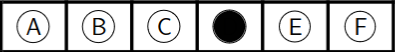
\includegraphics[scale=1.5]{images/00_answer_correct.png}};
\end{tikzpicture}

\begin{tikzpicture}[remember picture,overlay,shift={(current page.north east)}]
\node[anchor=north east,xshift=-1.7cm,yshift=-4.6cm]{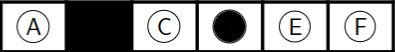
\includegraphics[scale=1.5]{images/00_answer_corrected.png}};
\end{tikzpicture}

\begin{tikzpicture}[remember picture,overlay,shift={(current page.north east)}]
\node[anchor=north east,xshift=-1.7cm,yshift=-7.0cm]{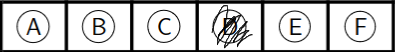
\includegraphics[scale=1.5]{images/00_answer_incorrect_1.png}};
\end{tikzpicture}

\begin{tikzpicture}[remember picture,overlay,shift={(current page.north east)}]
\node[anchor=north east,xshift=-1.7cm,yshift=-8.0cm]{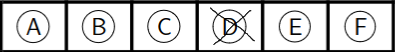
\includegraphics[scale=1.5]{images/00_answer_incorrect_2.png}};
\end{tikzpicture}

% remove space between top table and three bottom tables
\vspace{-1.5cm}


\def\tablebreak{0.5cm}
\def\tablebreaksmall{0.3cm}
\def\tablebreakbig{0.25cm}
\def\partanswers{& \circled{A} & \circled{B} & \circled{C} & \circled{D} & \circled{E}}

\begin{table}[H]
  \centering
  \begin{tabular}{
  M{\tablebreaksmall}|M{\tablebreak}|M{\tablebreak}|M{\tablebreak}|M{\tablebreak}|M{\tablebreak}|M{\tablebreakbig}M{\tablebreaksmall}|M{\tablebreak}|M{\tablebreak}|M{\tablebreak}|M{\tablebreak}|M{\tablebreak}|M{\tablebreakbig}M{\tablebreaksmall}|M{\tablebreak}|M{\tablebreak}|M{\tablebreak}|M{\tablebreak}|M{\tablebreak}|}
    \cline{2-6} \cline{9-13} \cline{16-20}
    1.\partanswers & & 21. \partanswers & & 41. \partanswers \\ \cline{2-6} \cline{9-13} \cline{16-20}
    2.\partanswers & & 22. \partanswers & & 42. \partanswers  \\ \cline{2-6} \cline{9-13} \cline{16-20}
    3.\partanswers & & 23. \partanswers & & 43. \partanswers  \\ \cline{2-6} \cline{9-13} \cline{16-20}
    4.\partanswers & & 24. \partanswers & & 44. \partanswers  \\ \cline{2-6} \cline{9-13} \cline{16-20}
    5.\partanswers & & 25. \partanswers & & 45. \partanswers  \\ \cline{2-6} \cline{9-13} \cline{16-20}
    6.\partanswers & & 26. \partanswers & & 46. \partanswers  \\ \cline{2-6} \cline{9-13} \cline{16-20}
    7.\partanswers & & 27. \partanswers & & 47. \partanswers  \\ \cline{2-6} \cline{9-13} \cline{16-20}
    8.\partanswers & & 28. \partanswers & & 48. \partanswers  \\ \cline{2-6} \cline{9-13} \cline{16-20}
    9.\partanswers & & 29. \partanswers & & 49. \partanswers  \\ \cline{2-6} \cline{9-13} \cline{16-20}
    10.\partanswers & & 30. \partanswers & & 50. \partanswers  \\ \cline{2-6} \cline{9-13} \cline{16-20}
    11.\partanswers & & 31. \partanswers & & 51. \partanswers  \\ \cline{2-6} \cline{9-13} \cline{16-20}
    12.\partanswers & & 32. \partanswers & & 52. \partanswers  \\ \cline{2-6} \cline{9-13} \cline{16-20}
    13.\partanswers & & 33. \partanswers & & 53. \partanswers  \\ \cline{2-6} \cline{9-13} \cline{16-20}
    14.\partanswers & & 34. \partanswers & & 54. \partanswers  \\ \cline{2-6} \cline{9-13} \cline{16-20}
    15.\partanswers & & 35. \partanswers & & 55. \partanswers  \\ \cline{2-6} \cline{9-13} \cline{16-20}
    16.\partanswers & & 36. \partanswers & & 56. \partanswers  \\ \cline{2-6} \cline{9-13} \cline{16-20}
    17.\partanswers & & 37. \partanswers & & 57. \partanswers  \\ \cline{2-6} \cline{9-13} \cline{16-20}
    18.\partanswers & & 38. \partanswers & & 58. \partanswers  \\ \cline{2-6} \cline{9-13} \cline{16-20}
    19.\partanswers & & 39. \partanswers & & 59. \partanswers  \\ \cline{2-6} \cline{9-13} \cline{16-20}
    20.\partanswers & & 40. \partanswers & & 60. \partanswers  \\ \cline{2-6} \cline{9-13} \cline{16-20}
  \end{tabular}
\end{table}

\begin{tikzpicture}[remember picture,overlay,shift={(current page.south west)}]
\node[anchor=south west,xshift=0.4cm,yshift=0.4cm]{
\includegraphics[scale=0.3]{images/markerBL.png}};
\end{tikzpicture}
\begin{tikzpicture}[remember picture,overlay,shift={(current page.south east)}]
\node[anchor=south east,xshift=-0.4cm,yshift=0.4cm]{
\includegraphics[scale=0.3]{images/markerBR.png}};
\end{tikzpicture}

\end{document}
